%
% beugung-herleitung.tex -- Herleitung aus WsComm2-Vorlesung
%
%
% !TEX root = ../../buch.tex
% !TEX encoding = UTF-8
%

\section{Anwendungsbeispiel}
\kopfrechts{Anwendungsbeispiel}

In der Drahtloskommunikation werden die Fresnel-Integrale für 
die Beugung von Signalen an einer sogenannten Knife-Edge gebraucht.
Diese Knife-Edge ragt als Hindernis zwischen zwei Antennen in die direkte 
Linie von Sender und Empfänger. 
Nun wird jede ausgesendete Welle als Kugelwelle angesehen,
welche sich nach Huygens kreisförmig ausbreitet. 
Um die Beugung zu berechnen, 
bedarf es einiger Definitionen, 
welche im weiteren Verlauf verwendet werden und in 
Abbildung~\ref{fresnel:Diff-loss-einseitig-abb} ersichtlich sind:
\begin{itemize}
    \item 
    $d$ sei der Abstand vom Empfänger zur Knife-Edge
    \item 
    $h$ sei die Höhe einer Kugelwelle direkt über der Knife-Edge
    \item
    $h_{\text{edge}}$ sei die Höhe, welche die Knife-Edge in die direkte Linie zwischen Sender und Empfänger hineinragt
    \item 
    $r$ sei die Distanz einer Kugelwelle zum Empfänger
\end{itemize}

\begin{figure}
    \centering
    % 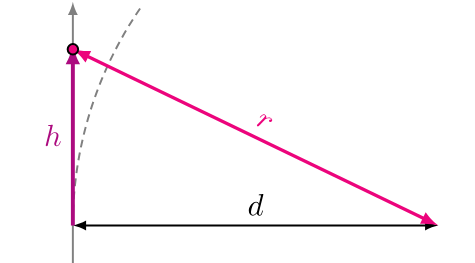
\includegraphics[width=0.8\linewidth]{papers/fresnel/images/Pythagoras-Dreieck.png}
     \resizebox{.7\textwidth}{!}{\input{papers/fresnel/images/Diff-Loss_einseitig.tex}\unskip}
    \caption{
        Darstellung der einseitigen Verlustberechnung
        \label{fresnel:Diff-loss-einseitig-abb}
    }
\end{figure}

\subsection{Fresnel-Integrale}
Die Fresnel-Integrale werden hier in der Form
\begin{equation}
    C(v) 
    = 
    \int_{0}^{v} \cos \left(\frac{\pi}{2}t^2\right)
    \quad \text{und} \quad
    S(v) 
    = 
    \int_{0}^{v} \sin \left(\frac{\pi}{2}t^2\right)
    \label{fresnel:integral-C-S-beispiel}
\end{equation}
definiert, wobei
\[
C(\infty)
=
S(\infty)
=
\frac{1}{2}
\quad
\text{und}
\quad
C(-a)
=
-C(a)
\quad
\text{sowie}
S(-a)
=
-S(a)
\]
sei.

\subsection{Fresnel Approximation}
Mittels Pythagoras geht hervor, dass 
\[
r 
= 
\sqrt{d^2 + h^2}
=
d \sqrt{1 + \frac{h^2}{d^2}}
\]
und mittels Taylor-Approximation für $d \gg h$
\[
r 
=
d \sqrt{1 + \frac{h^2}{d^2}}
\sim
d \left( 1 + \frac{h^2}{2d^2} \right)
=
d + \frac{h^2}{2d},
\]
unter der Annahme, dass in den meisten Fällen die Distanz zur Knife-Edge um ein Vielfaches grösser ist,
als die Höhe der Kugelwelle.
Will man nun das Signal zweier ankommender Kugelwellen am Empfänger berechnen, geht dies durch Einsetzen
\begin{align*}
    \text{für } h = 0: \quad \psi_0
    &=
    \psi \cdot \frac{e^{-jkr_0}}{r_0}
    =
    \psi \cdot \frac{e^{-jkd}}{d},
    \\
    \text{für } h > 0: \quad \psi_1
    &=
    \psi \cdot \frac{\text{exp}\left(-jkr_1\right)}{r_1}
    \approx
    \psi \cdot \frac{\text{exp}\left(-jk\left(d+\frac{h^2}{2d}\right)\right)}{d}.
\end{align*}
Da dieses Vorgehen eine Approximation ist, 
werden Abschwächungen und Verzögerungen der Signale vernächlässigt
$\to$ keine Faktoren wie $1/r, 1/d$ und $\omega t$. Daraus ergibt sich
\[
\psi (r,t)
=
\psi_0 \cdot \frac{e^{j(\omega t - kr)}}{r}
\quad \to \quad
\psi_0 \cdot e^{-jkr}
=
\psi (r)
\]
und kann für Kugelwellen in verschiedenen Höhen mit $h = h_i$ als
\begin{equation}
    \psi_i
    =
    \psi \cdot \text{exp}\left(-jkr\right)
    \approx
    \psi \cdot \text{exp}\left(-jk\left(d+\frac{h^2_i}{2d}\right)\right)
    \label{fresnel:Kugelwellen-signalstaerke}
\end{equation}
dargestellt werden. Mittels Superposition folgt
\begin{equation}
    \psi_{rx}
    =
    \sum_i \psi_i
    =
    \sum_i \psi \cdot e^{-jkr}
    =
    \psi \cdot \sum_i \text{exp}\left(-jk\left(d+\frac{h^2_i}{2d}\right)\right)
    =
    \underbrace{\psi \cdot e^{-jkd}}_{=\psi_0} \sum_i \text{exp}\left(-jk\left(\frac{h^2_i}{2d}\right)\right)
    \label{fresnel:Kugelwellen-signalstaerke-superpos}
\end{equation}
und mittels Wellendichte $\rho_{\psi} = \frac{d\psi}{dh} \Rightarrow \psi = \rho_{\psi} \Delta h $
\begin{equation}
    \psi_{rx}
    =
    \psi_0 \cdot \sum_i \text{exp}\left(-jk\left(\frac{h^2_i}{2d}\right)\right)
    =
    \rho_{\psi_0} \cdot \sum_i \text{exp}\left(-jk\left(\frac{h^2_i}{2d}\right)\right) \Delta h,
    \label{fresnel:Kugelwellen-wellendichte}
\end{equation}
welches anschliessend mittels $\Delta h \to dh$ zum Integral
\begin{equation}
    \psi_{rx}
    =
    \rho_{\psi_0} \int_{h_{\text{edge}}}^{\infty} \text{exp}\left(-jk\left(\frac{h^2}{2d}\right)\right) dh
    =
    \rho_{\psi_0} \int_{h_{\text{edge}}}^{\infty} \left(\cos \frac{kh^2}{2d} - j \sin \frac{kh^2}{2d}\right) dh
    \label{fresnel:Kugelwellen-wellendichte-integral}
\end{equation}
wird.
Dies kann mit den gängigen Regeln in zwei Integrale mit Beginn bei 0 umgestellt werden, was zu
\begin{align*}
    \psi_{rx}
    &=
    \rho_{\psi_0} \int_{h_{\text{edge}}}^{\infty} \left(\cos \frac{kh^2}{2d} - j \sin \frac{kh^2}{2d}\right) dh
    \\
    &=
    \underbrace{\rho_{\psi_0} \int_{0}^{\infty} \left(\cos \frac{kh^2}{2d} - j \sin \frac{kh^2}{2d}\right) dh}_{\text{Gesamte Wellendichte}}
    -
    \underbrace{\rho_{\psi_0} \int_{0}^{h_{\text{edge}}} \left(\cos \frac{kh^2}{2d} - j \sin \frac{kh^2}{2d}\right) dh}_{\text{Verlorene Wellendichte durch Knife-Edge}}  
\end{align*}
führt.
Das Integral ähnelt $C$ aus der Formel~\eqref{fresnel:integral-C-S-beispiel} und kann mittels der Substitution
\[
h
\to
t(h)
=
h\sqrt{\frac{h}{\pi d}}
\Rightarrow
\frac{dh}{dt}
=
\sqrt{\frac{\pi d}{k}}
\Rightarrow
dh
=
\sqrt{\frac{\pi d}{k}} dt
\]
aufgelöst werden zu
\begin{equation*}
    \int_{0}^{h_{\text{edge}}} \cos \left(\frac{k}{2d}h^2\right) dh
    =
    \sqrt{\frac{\pi d}{k}} \int_{0}^{h_{\text{edge}}\sqrt{\frac{k}{\pi d}}} \cos \left(\frac{\pi}{2}t^2\right) dt
    =
    \sqrt{\frac{\pi d}{k}} C(v).
\end{equation*}
Über das ganze Integral ergibt sich
\begin{equation}
    \psi_{rx} (v)
    =
    \rho_{\psi_0} \sqrt{\frac{\pi d}{k}} \cdot \left[\frac{1}{2} - C(v) -j\left(\frac{1}{2}-S(v)\right)\right]
\end{equation}
mit dem daraus entstehenden Fresnel-Parameter
\begin{equation}
    v
    =
    h_{\text{edge}} \sqrt{\frac{k}{\pi d}}
    \quad
    \overset{k = \frac{2 \pi}{\lambda}}{=}
    \quad
    h_{\text{edge}} \sqrt{\frac{2}{\lambda d}}.
\end{equation}

\subsection{Beugungsverlust}
Aus den hervorgehenden Gleichungen kann der Beugungsverlust $L(v)$ berechnet werden,
indem das Verhältnis der gesamten Signalstärke zur verlorenen Signalstärke berechnet wird.
In der Elektrotechnik werden Verhältnisse immer zwischen Leistungen und nicht zwischen Signalen berechnet,
weshalb in
\begin{equation}
    L(v)
    =
    \frac{|\psi_{rx} (-\infty)|^2}{|\psi_{rx} (v)|^2}
    =
    \dots
    =
    \frac{2}{\left|\frac{1}{2}-C(v)\right|^2 + \left|\frac{1}{2}-S(v)\right|^2}
    \label{fresnel:diff-loss-einseitig}
\end{equation}
bei den Signalen die Beträge und anschliessend das Quadrat davon verwendet wird.
Aus dem Verhältnis lässt sich dann der Verlust $L_{\unit{\decibel}}$ mit der Umformung
\[
L_{\unit{\decibel}} (v)
=
10 \cdot \log_{10}L(v)
\]
berechnen.
Die Gleichung \eqref{fresnel:diff-loss-einseitig} gilt für Verluste zwischen Knife-Edge und Empfänger. 
Soll nun der Beugungsverlust zwischen Sender und Empfänger 
mit dazwischenliegender Knife-Edge wie in Abbildung~\ref{fresnel:knife-edge-abb} berechnet
werden, folgt
\[
r
=
r_1 + r_2
\quad
\text{mit}
\quad
r_n
=
\sqrt{d_n^2 + h^2}
=
d_n \sqrt{1 + \frac{h^2}{d_n^2}}
\text{ für }
n = {1,2}.
\]
Wir nehmen wie im vorherigen Abschnitt an, 
dass die Distanzen bedeutend grösser sind als die Höhe der Knife-Edge ($d \gg h$)
und können dank der Taylor-Approximation den Term von $r_n $ zu
\[
r_n
=
d_n \sqrt{1 + \frac{h^2}{d_n^2}}
\approx
d_n + \frac{h^2}{2d_n}
\]
vereinfachen und erhalten damit die gesamte Distanz $r$ mit
\[
r
\approx
d_1 + d_2 + \frac{h^2}{2}\left(\frac{1}{d_1} + \frac{1}{d_2}\right)
=
d_1 + d_2 + h^2\left(\frac{d_1 + d_2}{2d_1d_2}\right).
\]
Setzt man die neue Distanz $r$ in die Gleichung \eqref{fresnel:Kugelwellen-signalstaerke-superpos} ein, folgt
\begin{equation}
    \psi_{rx}
    =
    \psi \cdot \sum_i \text{exp}\left(-jk\left(d_1 + d_2 + h^2_i\frac{d_1 + d_2}{2d_1d_2}\right)\right)
    =
    \underbrace{\psi \cdot e^{-jk(d_1 + d_2)}}_{=\psi_0} \sum_i \text{exp}\left(-jk\left(h^2_i\frac{d_1 + d_2}{2d_1d_2}\right)\right).
    \label{fresnel:Kugelwellen-signalstaerke-superpos-beidseitig}
\end{equation}
Unter genauer Betrachtung fällt auf,
dass die neue Gleichung \eqref{fresnel:Kugelwellen-signalstaerke-superpos-beidseitig} der vorherigen stark gleicht.
Im Grunde ändert sich lediglich der Parameter
\[
\frac{1}{d}
\text{ zu }
\frac{d_1 + d_2}{d_1d_2},
\]
welches folglich auf den Fresnel-Parameter $v$ anhand
\begin{equation}
    v
    =
    h_{\text{edge}} \sqrt{2\frac{d_1 + d_2}{\lambda d_1 d_2}}
\end{equation}
angewendet werden kann.
% Parameter bleibt, wenn einer der Stationen viel weiter vom Knife-Edge weg ist, als der andere

\begin{figure}
    \centering
    % 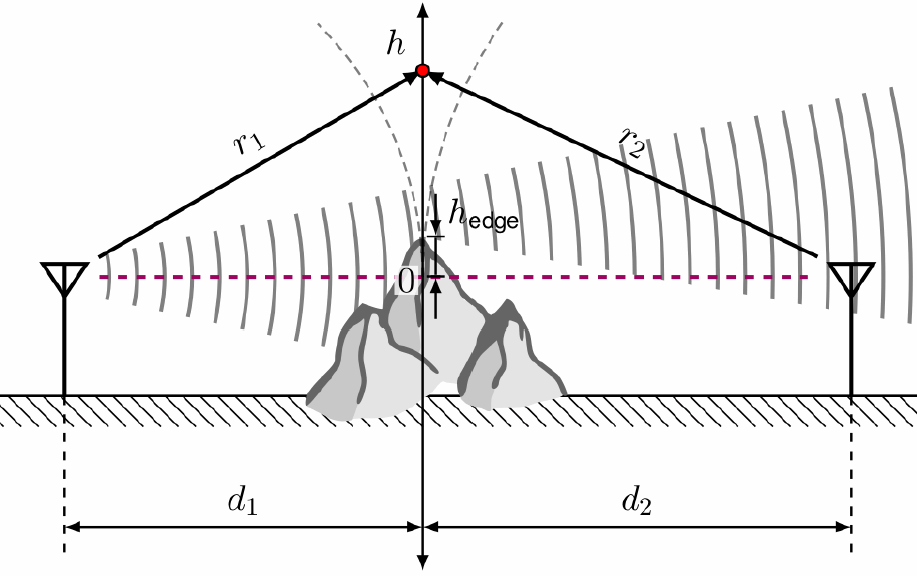
\includegraphics[width=0.8\linewidth]{papers/fresnel/images/Diff-Loss_beidseitig.png}
    \resizebox{.8\textwidth}{!}{\input{papers/fresnel/images/Diff-Loss_beidseitig.tex}\unskip}
    \caption{
        Darstellung der Knife-Edge zwischen Sender und Empfänger
        \label{fresnel:knife-edge-abb}
    }
\end{figure}

Die daraus resultierenden Verluste $L_{\unit{\decibel}}$ können aus Abbildung~\ref{fresnel:Fresnel-Diagram}
ausgelesen oder mit den Formeln
\begin{subequations}
    \begin{align}
        v > 1: \quad
        -L_{\unit{\decibel}}
        &=
        20 \log_{10}v + \qty{13}{\decibel}
        \\
        v > -0.7: \quad
        -L_{\unit{\decibel}}
        &=
        20 \log_{10}\left(\sqrt{(v-0.1)^2 + 1} + v -0.1\right) + \qty{6.9}{\decibel}
        \\
        \text{sonst:} \quad
        -L_{\unit{\decibel}}
        &=
        10 \log_{10} L(v)
    \end{align}
\end{subequations}
angenähert werden.

\begin{figure}
    \centering
    % 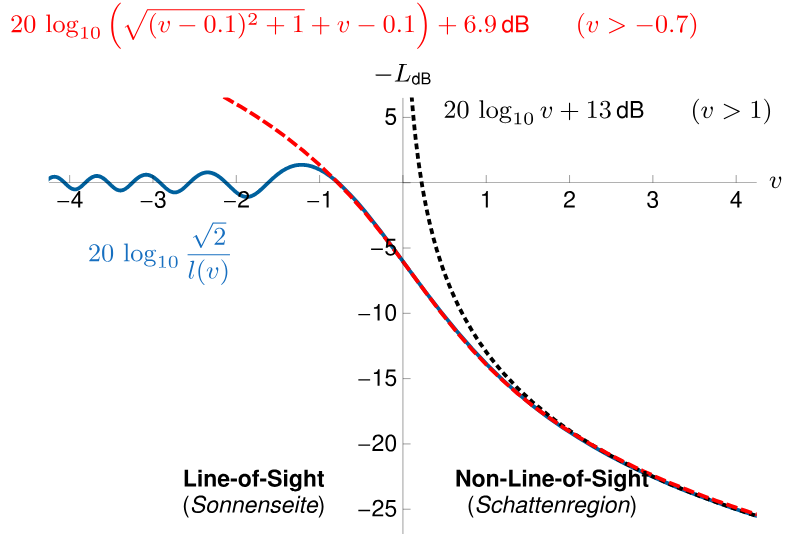
\includegraphics[width=0.8\linewidth]{papers/fresnel/images/Fresnel-Diagram.png}
    \resizebox{0.85\textwidth}{!}{\input{papers/fresnel/pgf/beugungsverluste.pgf}\unskip}
    \caption{
        Diagramm Fresnel-Parameter und Verluste
        \label{fresnel:Fresnel-Diagram}
    }
\end{figure}